\documentclass{beamer}
\usetheme{Amurmaple}
\usepackage{graphicx}
\usepackage[table,xcdraw]{xcolor} % Allows for table coloring
\usepackage{colortbl} % Allows table border coloring
\usepackage{amsthm}
\usepackage{wrapfig}
\usepackage[dvipsnames]{xcolor}
\usepackage{tikz}
\usepackage{subcaption} % For subfigure environment
% \documentclass[tikz,border=2mm]{standalone}
\usetikzlibrary{arrows.meta,positioning}

\title{Nash Equilibrium}
\subtitle{Using Beamer}
\author{Arnab Sarker \& Enayet Alvee}
% \text {2105099  \& 2105107}
\institute{Bangladesh University of Engineering and Technology}
\date{\today}

\begin{document}

\maketitle

\section{}

\begin{frame}
    \frametitle{\centering Story} % Centers the frame title
    \vfill % Pushes content down
        \begin{center}
        {\LARGE Let's Start with a Story} % Centers and enlarges the text
    \end{center}

    \vfill % Adds space below
\end{frame}

\begin{frame}
        \begin{columns}[c] % Creates two columns
        \column{0.5\textwidth} % First column taking half width
        
\includegraphics[width=\textwidth]{Image/Honda.jpg} % Replace 'path_to_image1' with your image file path

        \column{0.5\textwidth} % Second column taking half width
        
\includegraphics[width=\textwidth]{Image/Toyota.jpg} % Replace 'path_to_image2' with your image file path
    \end{columns}
\end{frame}






\begin{frame}{Table}

\only<1>{
\begin{table}[]
\begin{tabular}{|
>{\columncolor[HTML]{F56B00}}c 
>{\columncolor[HTML]{F56B00}}c |
>{\columncolor[HTML]{F8FF00}}l 
>{\columncolor[HTML]{F8FF00}}l |}
\hline
\multicolumn{2}{|c|}{\cellcolor[HTML]{F56B00}{\color[HTML]{000000} }} & \multicolumn{2}{c|}{\cellcolor[HTML]{FD6864}{\color[HTML]{000000} TOYOTA Company}} \\ \cline{3-4} 
\multicolumn{2}{|c|}{\cellcolor[HTML]{F56B00}{\color[HTML]{000000} \begin{tabular}[c]{@{}c@{}}Profit\\ IN\\ Millions\end{tabular}}} &
  \multicolumn{1}{c|}{\cellcolor[HTML]{38FFF8}Building new plant} &
  \multicolumn{1}{c|}{\cellcolor[HTML]{38FFF8}\begin{tabular}[c]{@{}c@{}}Not Building \\ plant\end{tabular}} \\ \hline
\cellcolor[HTML]{FD6864}{\color[HTML]{000000} HONDA} &
  \cellcolor[HTML]{38FFF8}\begin{tabular}[c]{@{}c@{}}Building  new  \\ plant\end{tabular} &
  \multicolumn{1}{l|}{\cellcolor[HTML]{EFEFEF}{\color[HTML]{000000} 16                 16}} &
  {\color[HTML]{000000}                   } \\ \hline
\cellcolor[HTML]{FD6864} &
  \cellcolor[HTML]{38FFF8}\begin{tabular}[c]{@{}c@{}}Not Building new\\ plant\end{tabular} &
  \multicolumn{1}{l|}{\cellcolor[HTML]{EFEFEF}                 } &
                     \\ \hline
\end{tabular}
\end{table}
}

\only<2>{
\begin{table}[]
\begin{tabular}{|
>{\columncolor[HTML]{F56B00}}c 
>{\columncolor[HTML]{F56B00}}c |
>{\columncolor[HTML]{F8FF00}}l 
>{\columncolor[HTML]{F8FF00}}l |}
\hline
\multicolumn{2}{|c|}{\cellcolor[HTML]{F56B00}{\color[HTML]{000000} }} & \multicolumn{2}{c|}{\cellcolor[HTML]{FD6864}{\color[HTML]{000000} TOYOTA Company}} \\ \cline{3-4} 
\multicolumn{2}{|c|}{\cellcolor[HTML]{F56B00}{\color[HTML]{000000} \begin{tabular}[c]{@{}c@{}}Profit\\ IN\\ Millions\end{tabular}}} &
  \multicolumn{1}{c|}{\cellcolor[HTML]{38FFF8}Building new plant} &
  \multicolumn{1}{c|}{\cellcolor[HTML]{38FFF8}\begin{tabular}[c]{@{}c@{}}Not Building \\ plant\end{tabular}} \\ \hline
\cellcolor[HTML]{FD6864}{\color[HTML]{000000} HONDA} &
  \cellcolor[HTML]{38FFF8}\begin{tabular}[c]{@{}c@{}}Building  new  \\ plant\end{tabular} &
  \multicolumn{1}{l|}{\cellcolor[HTML]{EFEFEF}{\color[HTML]{000000} 16                 16}} &
  {\color[HTML]{000000}  15               20} \\ \hline
\cellcolor[HTML]{FD6864} &
  \cellcolor[HTML]{38FFF8}\begin{tabular}[c]{@{}c@{}}Not Building new\\ plant\end{tabular} &
  \multicolumn{1}{l|}{\cellcolor[HTML]{EFEFEF}                 } &
                     \\ \hline
\end{tabular}
\end{table}
}


\only<3>{
\begin{table}[]
\begin{tabular}{|
>{\columncolor[HTML]{F56B00}}c 
>{\columncolor[HTML]{F56B00}}c |
>{\columncolor[HTML]{F8FF00}}l 
>{\columncolor[HTML]{F8FF00}}l |}
\hline
\multicolumn{2}{|c|}{\cellcolor[HTML]{F56B00}{\color[HTML]{000000} }} & \multicolumn{2}{c|}{\cellcolor[HTML]{FD6864}{\color[HTML]{000000} TOYOTA Company}} \\ \cline{3-4} 
\multicolumn{2}{|c|}{\cellcolor[HTML]{F56B00}{\color[HTML]{000000} \begin{tabular}[c]{@{}c@{}}Profit\\ IN\\ Millions\end{tabular}}} &
  \multicolumn{1}{c|}{\cellcolor[HTML]{38FFF8}Building new plant} &
  \multicolumn{1}{c|}{\cellcolor[HTML]{38FFF8}\begin{tabular}[c]{@{}c@{}}Not Building \\ plant\end{tabular}} \\ \hline
\cellcolor[HTML]{FD6864}{\color[HTML]{000000} HONDA} &
  \cellcolor[HTML]{38FFF8}\begin{tabular}[c]{@{}c@{}}Building  new  \\ plant\end{tabular} &
  \multicolumn{1}{l|}{\cellcolor[HTML]{EFEFEF}{\color[HTML]{000000} 16                 16}} &
  {\color[HTML]{000000}  15               20} \\ \hline
\cellcolor[HTML]{FD6864} &
  \cellcolor[HTML]{38FFF8}\begin{tabular}[c]{@{}c@{}}Not Building new\\ plant\end{tabular} &
  \multicolumn{1}{l|}{\cellcolor[HTML]{EFEFEF}20                 15} &
                     \\ \hline
\end{tabular}
\end{table}
}

\only<4>{
\begin{table}[]
\begin{tabular}{|
>{\columncolor[HTML]{F56B00}}c 
>{\columncolor[HTML]{F56B00}}c |
>{\columncolor[HTML]{F8FF00}}l 
>{\columncolor[HTML]{F8FF00}}l |}
\hline
\multicolumn{2}{|c|}{\cellcolor[HTML]{F56B00}{\color[HTML]{000000} }} & \multicolumn{2}{c|}{\cellcolor[HTML]{FD6864}{\color[HTML]{000000} TOYOTA Company}} \\ \cline{3-4} 
\multicolumn{2}{|c|}{\cellcolor[HTML]{F56B00}{\color[HTML]{000000} \begin{tabular}[c]{@{}c@{}}Profit\\ IN\\ Millions\end{tabular}}} &
  \multicolumn{1}{c|}{\cellcolor[HTML]{38FFF8}Building new plant} &
  \multicolumn{1}{c|}{\cellcolor[HTML]{38FFF8}\begin{tabular}[c]{@{}c@{}}Not Building \\ plant\end{tabular}} \\ \hline
\cellcolor[HTML]{FD6864}{\color[HTML]{000000} HONDA} &
  \cellcolor[HTML]{38FFF8}\begin{tabular}[c]{@{}c@{}}Building  new  \\ plant\end{tabular} &
  \multicolumn{1}{l|}{\cellcolor[HTML]{EFEFEF}{\color[HTML]{000000} 16                 16}} &
  {\color[HTML]{000000}  15               20} \\ \hline
\cellcolor[HTML]{FD6864} &
  \cellcolor[HTML]{38FFF8}\begin{tabular}[c]{@{}c@{}}Not Building new\\ plant\end{tabular} &
  \multicolumn{1}{l|}{\cellcolor[HTML]{EFEFEF}20                 15} &
        18            18 \\ \hline
\end{tabular}
\end{table}
}
\end{frame}

\begin{frame}
        \only<1>{
        \begin{columns}[c] % Creates two columns
        \column{0.5\textwidth} % First column taking half width
        
\includegraphics[width=0.75\textwidth]{Image/Competator.jpg} 
    \end{columns}
    \begin{center}
    \Large Guess,Who will be the winner?    
    \end{center}
    }
    \only<2>{
    \begin{center}
    Before ending of this presentation,we will be able to know the answer
    \end{center}
    }
    
\end{frame}



\begin{frame}{Introduction to Nash Equilibrium}
    \only<1>{
    \begin{center}
        \Large The concept of Nash Equilibrium was created by John Nash, an American mathematician.
    \end{center}
    }
    \only<2>{
    \begin{center}
        \Large John Nash was awarded the Nobel Memorial Prize in Economic Sciences in 1994 for his contributions to game theory, including the concept of Nash Equilibrium.
    \end{center}
    }

    \only<3>{
    \begin{center}
            \Large Nash Equilibrium is a concept in game theory where each player chooses the best strategy, considering the strategies of others. It occurs when no player can improve their outcome by changing their own strategy, as long as the others stick to theirs. This idea helps to understand decision-making in situations where people or companies compete or cooperate. Nash Equilibrium explains how participants often reach a stable outcome even without directly communicating.
        
    \end{center}
    }
    

\end{frame}

\begin{frame}{Why Nash Equilibrium ?}
         \begin{columns}[c] % Creates two columns
        \column{1\textwidth} % First column taking half width
        
\includegraphics[width=\textwidth]{Image/ThinkingBoy.jpg} % Replace 'path_to_image1' with your image file path
    \end{columns}
\end{frame}

\begin{frame}{Why Nash Equilibrium ?}
         \begin{columns}[c] % Creates two columns
        \column{0.5\textwidth} % First column taking half width
        
\includegraphics[width=\textwidth]{Image/HappyBoy.jpg} % Replace 'path_to_image1' with your image file path
    \end{columns}
     Now I can take best decisions
    
\end{frame}

\begin{frame}{Why Nash Equilibrium ? }
\setbeamercovered{transparent} % Transparency for uncovered items

        \begin{itemize}
        \item      people make decisions 
        \item<2->  predicting outcomes 
        \item<3->  stable and predictable results.
        \item<4->  everyone could do better if they cooperated 
        \item<5->decision-making with interdependence
        \item<6->navigate conflicts and cooperation.

    \end{itemize}

\end{frame}

\begin{frame}
        \only<1>{
    \begin{center}
        \Large There are eight types of Nash Equilibrium based on different classifications in game theory.
    \end{center}
    }
    \only<2>{
    \begin{center}
        \Large We will discuss all categories of Nash Equilibrium. \\
        However, the first two types are the core categories, \\
        so we will talk about them in detail later.
    \end{center}
    }
\end{frame}




\begin{frame}{Types of Nash Equilibrium}
    \setbeamercovered{transparent} % Transparency for uncovered items
    \begin{itemize}
        \item  Pure Strategy Nash Equilibrium
        \item<2->Mixed Strategy Nash Equilibrium 
        \item<3->Symmetric Nash Equilibrium
        \item<4->Asymmetric Nash Equilibrium
        \item<5->Strict Nash Equilibrium
        \item<6->Weak Nash Equilibrium
        \item<7->Subgame Perfect Nash Equilibrium (SPNE)
        \item<8->Correlated Nash Equilibrium
    \end{itemize}
\end{frame}





\begin{frame}{Pure Strategy Nash Equilibrium}
     \setbeamercovered{transparent} % Transparency for uncovered items
    \begin{itemize}
        \item  All players in a game choose strategies with certainty. 
        \item<2->No player can improve their outcome by unilaterally changing their strategy.
        \item<3-> Maximizes their payoff given the strategies of others.
    \end{itemize}
    
\end{frame}

\begin{frame}{Pure Strategy Example}
    \only<1>{
     \begin{columns}[c] % Creates two columns
        \column{1\textwidth} % First column taking half width
        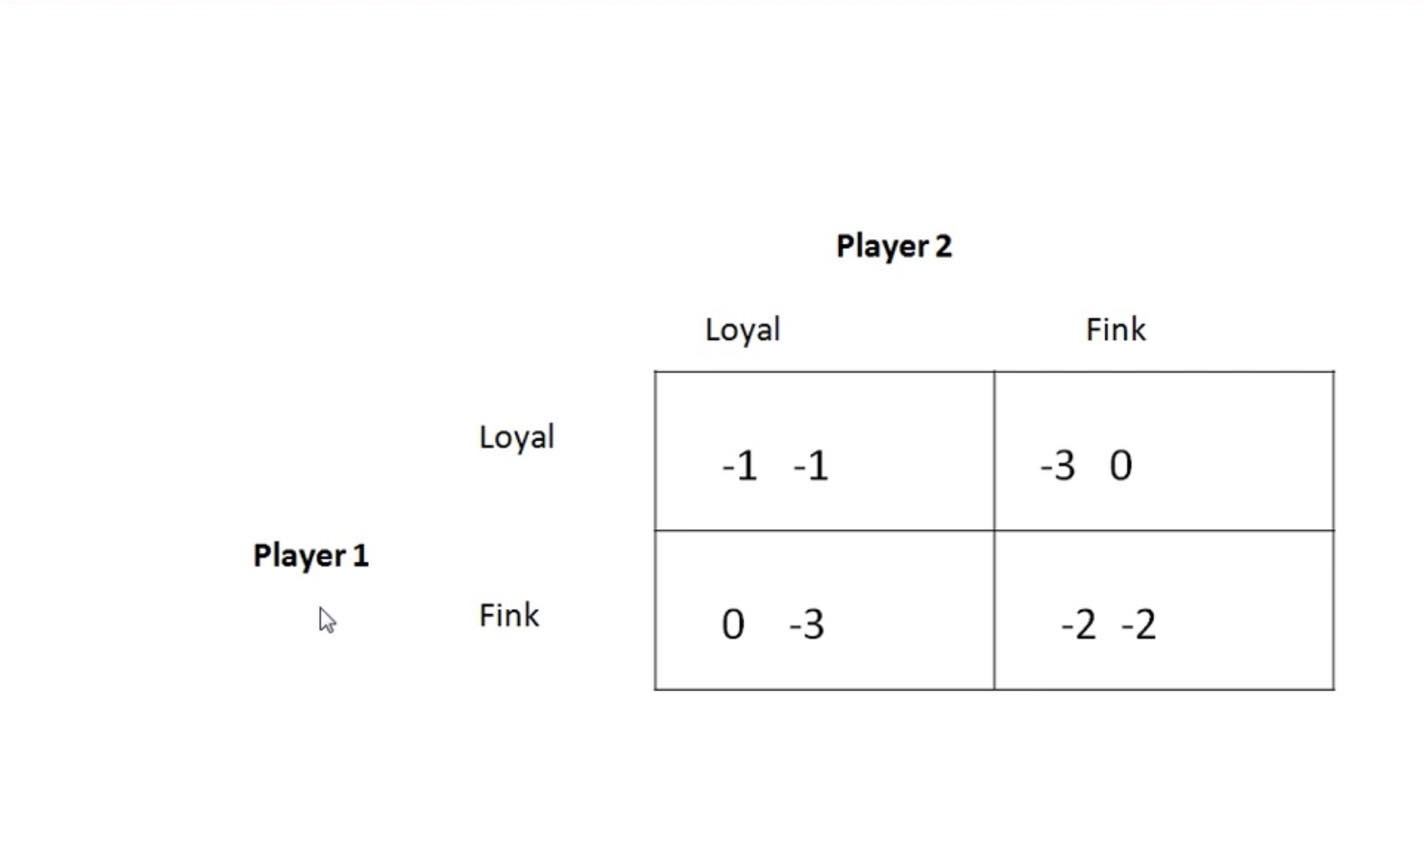
\includegraphics[width=\textwidth]{Image/ss1.jpg} 
    \end{columns}
    }

    \only<2>{
    \begin{columns}[c] % Creates two columns
        \column{1\textwidth} % First column taking half width
        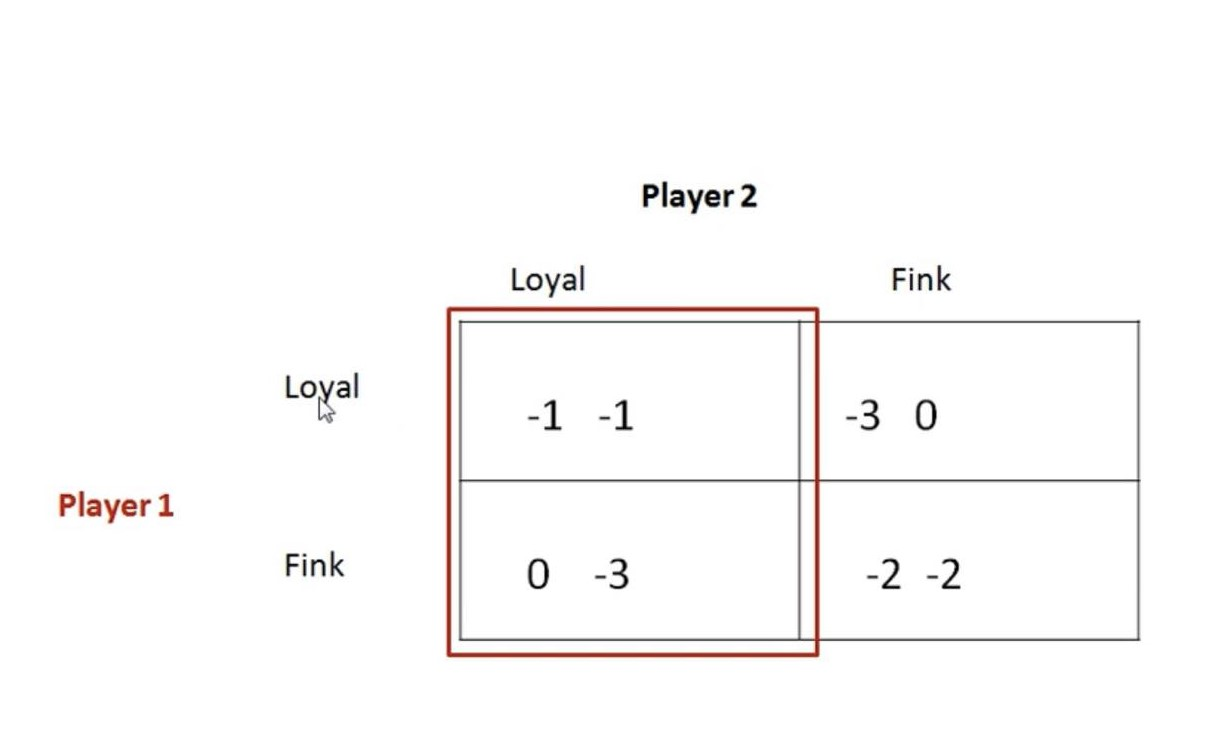
\includegraphics[width=\textwidth]{Image/ss2.jpg} 
    \end{columns}
    }

    \only<3>{
    \begin{columns}[c] % Creates two columns
        \column{1\textwidth} % First column taking half width
        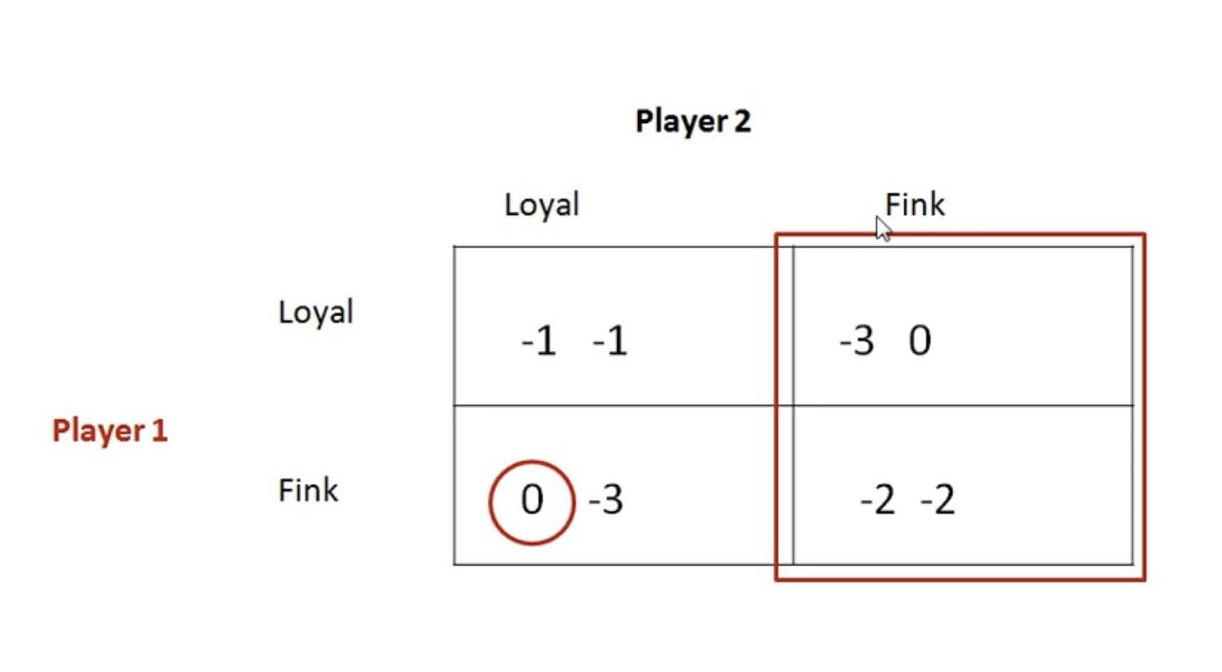
\includegraphics[width=\textwidth]{Image/ss3.jpg} 
    \end{columns}
    }
    \only<4>{
    \begin{columns}[c] % Creates two columns
        \column{1\textwidth} % First column taking half width
        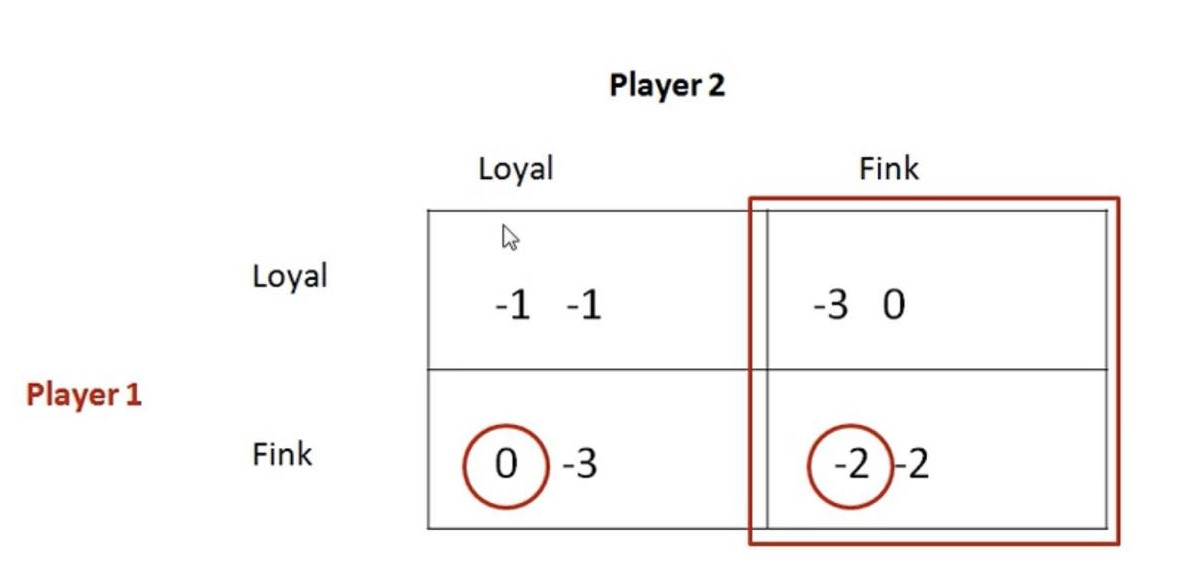
\includegraphics[width=\textwidth]{Image/ss4.jpg} 
    \end{columns}
    }
    \only<5>{
    \begin{columns}[c] % Creates two columns
        \column{1\textwidth} % First column taking half width
        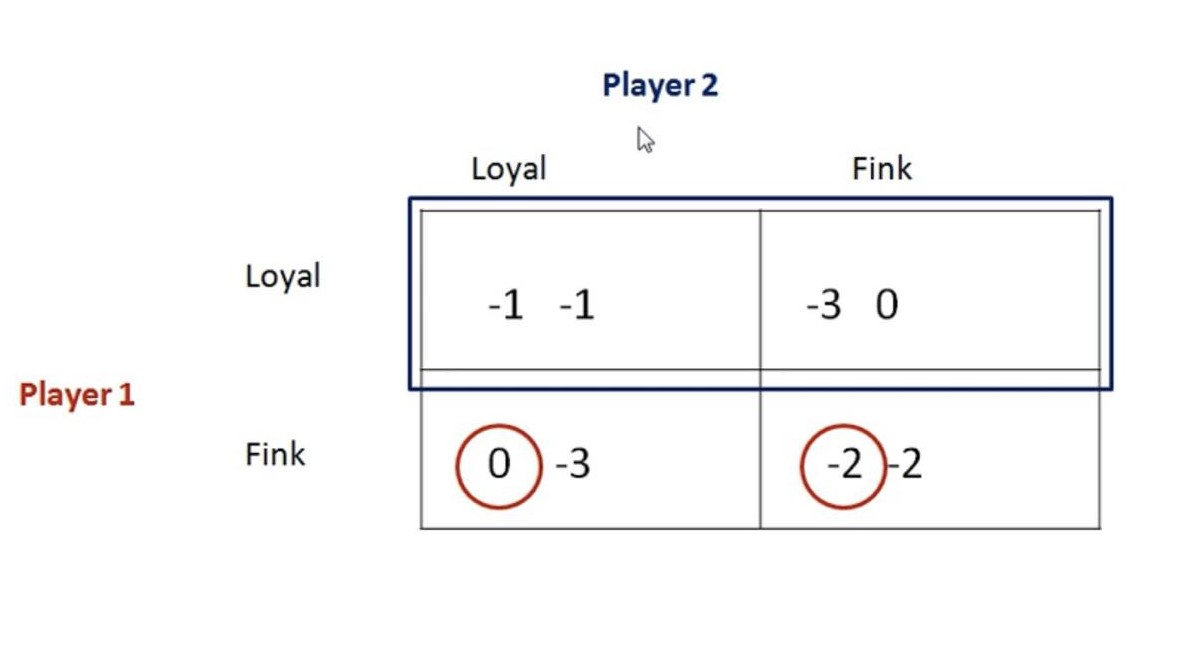
\includegraphics[width=\textwidth]{Image/ss5.jpg} 
    \end{columns}
    }
    \only<6>{
    \begin{columns}[c] % Creates two columns
        \column{1\textwidth} % First column taking half width
        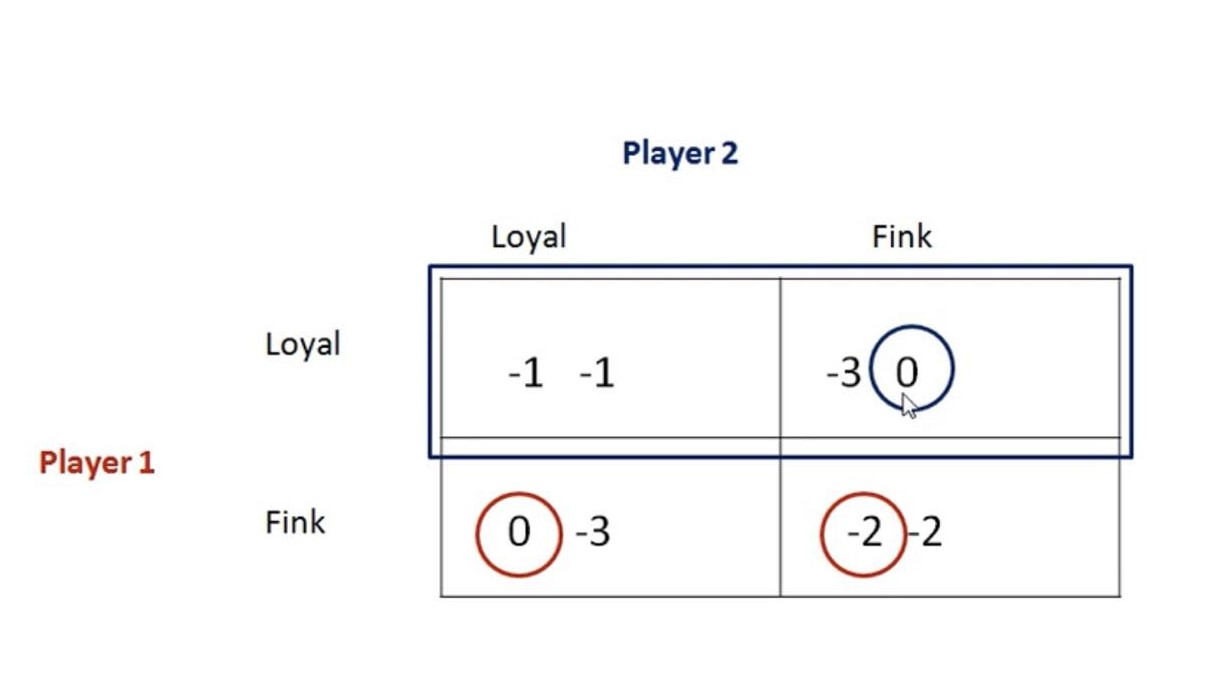
\includegraphics[width=\textwidth]{Image/ss6.jpg} 
    \end{columns}
    }
    \only<7>{
    \begin{columns}[c] % Creates two columns
        \column{1\textwidth} % First column taking half width
        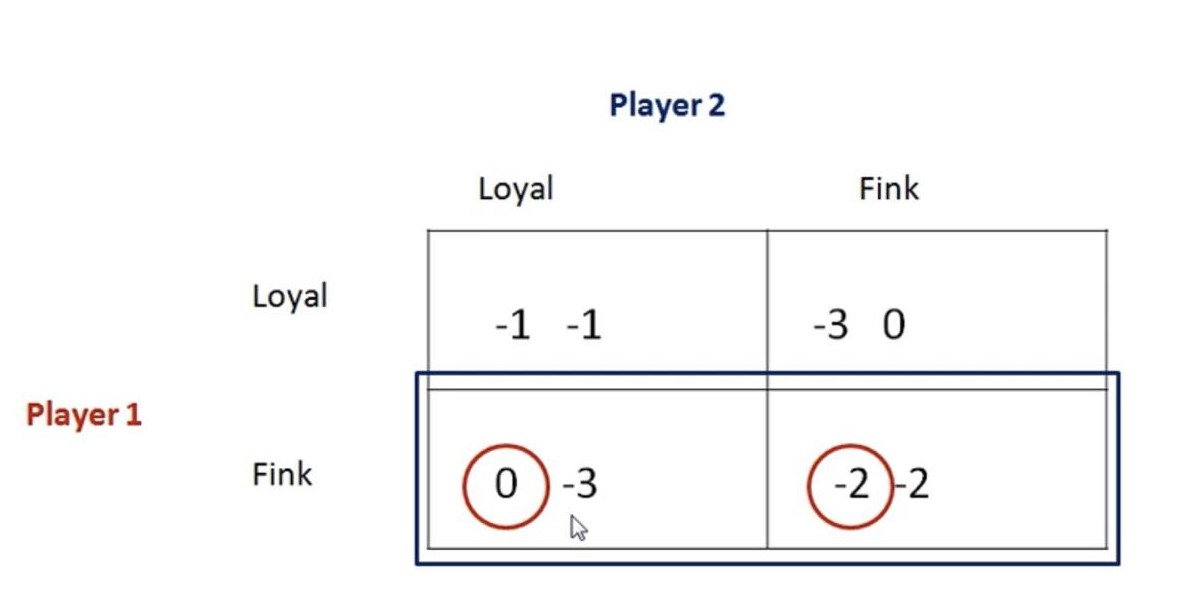
\includegraphics[width=\textwidth]{Image/ss7.jpg} 
    \end{columns}
    }
    \only<8>{
        \begin{columns}[c] % Creates two columns
        \column{1\textwidth} % First column taking half width
        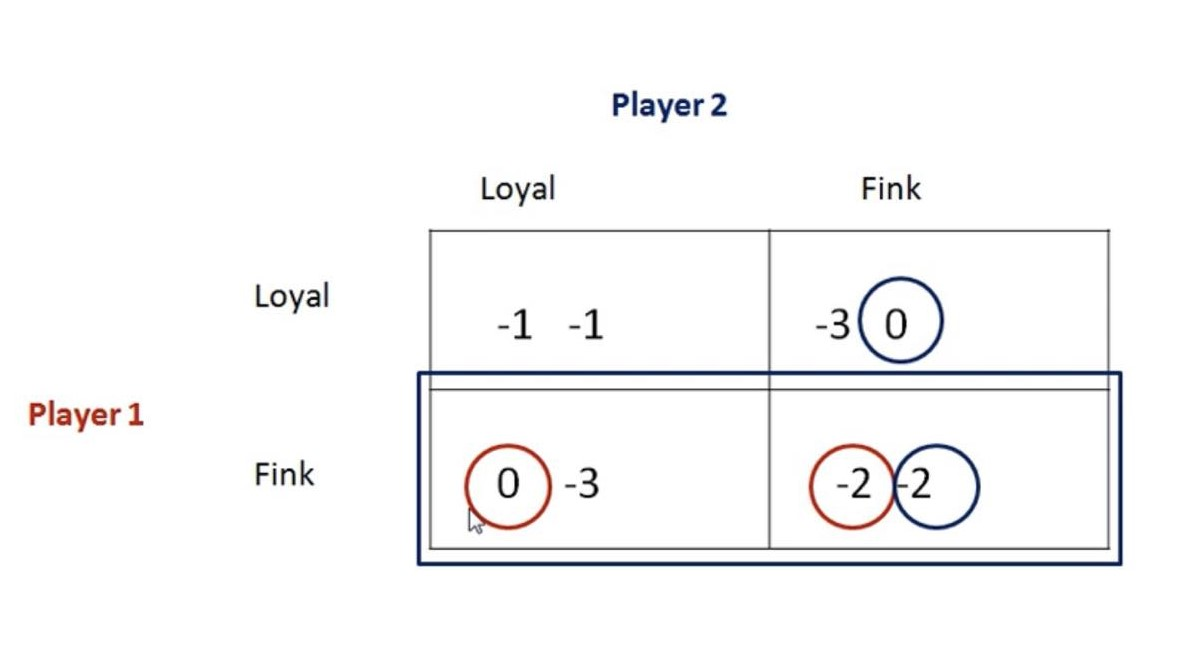
\includegraphics[width=\textwidth]{Image/ss8.jpg} 
    \end{columns}    
    }

    \only<9>{
    \begin{columns}[c] % Creates two columns
        \column{1\textwidth} % First column taking half width
        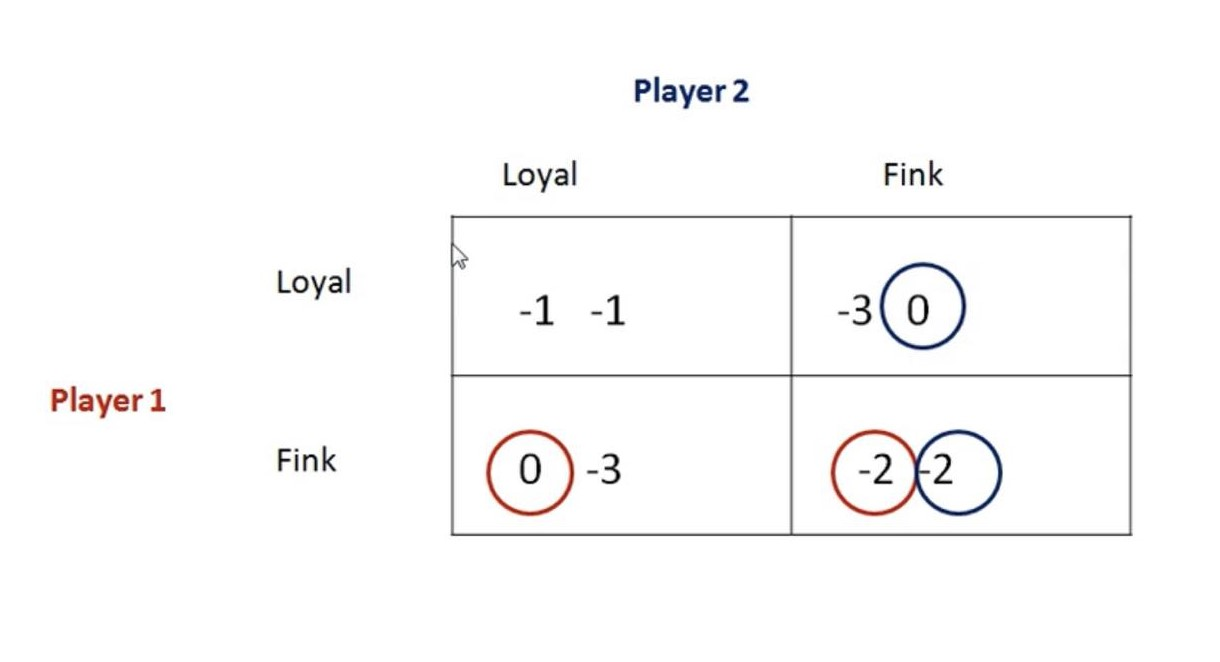
\includegraphics[width=\textwidth]{Image/ss9.jpg} 
    \end{columns}
    }

    \only<10>{
    \begin{table}[]
\begin{tabular}{|
>{\columncolor[HTML]{F56B00}}c 
>{\columncolor[HTML]{F56B00}}c |
>{\columncolor[HTML]{F8FF00}}l 
>{\columncolor[HTML]{F8FF00}}l |}
\hline
\multicolumn{2}{|c|}{\cellcolor[HTML]{F56B00}{\color[HTML]{000000} }} & \multicolumn{2}{c|}{\cellcolor[HTML]{FD6864}{\color[HTML]{000000} TOYOTA Company}} \\ \cline{3-4} 
\multicolumn{2}{|c|}{\cellcolor[HTML]{F56B00}{\color[HTML]{000000} \begin{tabular}[c]{@{}c@{}}Profit\\ IN\\ Millions\end{tabular}}} &
  \multicolumn{1}{c|}{\cellcolor[HTML]{38FFF8}Building new plant} &
  \multicolumn{1}{c|}{\cellcolor[HTML]{38FFF8}\begin{tabular}[c]{@{}c@{}}Not Building \\ plant\end{tabular}} \\ \hline
\cellcolor[HTML]{FD6864}{\color[HTML]{000000} HONDA} &
  \cellcolor[HTML]{38FFF8}\begin{tabular}[c]{@{}c@{}}Building  new  \\ plant\end{tabular} &
  \multicolumn{1}{l|}{\cellcolor[HTML]{EFEFEF}{\color[HTML]{000000} 16                 16}} &
  {\color[HTML]{000000}  15               20} \\ \hline
\cellcolor[HTML]{FD6864} &
  \cellcolor[HTML]{38FFF8}\begin{tabular}[c]{@{}c@{}}Not Building new\\ plant\end{tabular} &
  \multicolumn{1}{l|}{\cellcolor[HTML]{EFEFEF}20                 15} &
        18            18 \\ \hline
\end{tabular}
\end{table}
    }
\end{frame}



\begin{frame}{Mixed Nash Equilibrium Example}

    \only<1>{
    \begin{columns}[c] % Creates two columns
        \column{1\textwidth} % First column taking half width
        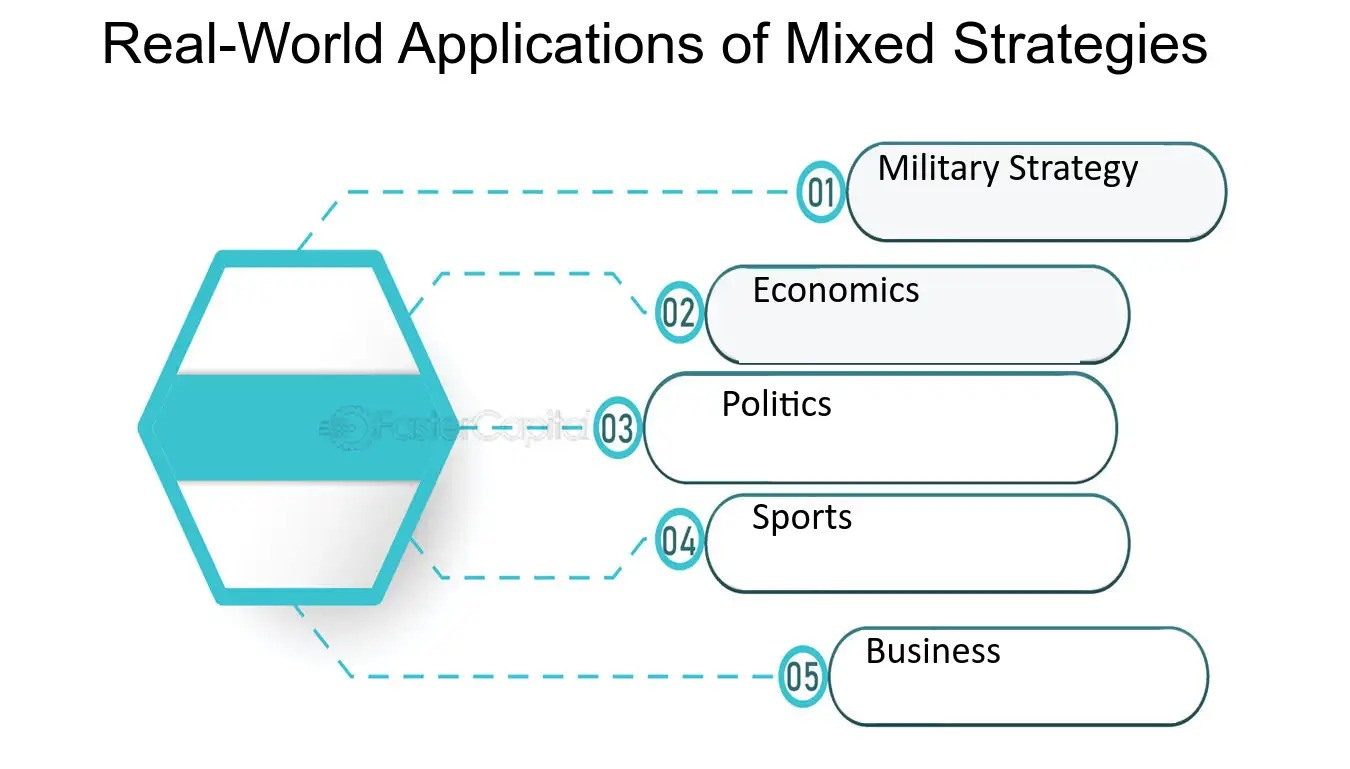
\includegraphics[width=\textwidth]{Image/Mixed Examples.jpg} 
    \end{columns}
    
    }
\end{frame}




\end{document}